% CVPR 2022 Paper Template
% based on the CVPR template provided by Ming-Ming Cheng (https://github.com/MCG-NKU/CVPR_Template)
% modified and extended by Stefan Roth (stefan.roth@NOSPAMtu-darmstadt.de)

\documentclass[10pt,twocolumn,letterpaper]{article}

%%%%%%%%% PAPER TYPE  - PLEASE UPDATE FOR FINAL VERSION
% \usepackage[review]{cvpr}      % To produce the REVIEW version
\usepackage{cvpr}              % To produce the CAMERA-READY version
%\usepackage[pagenumbers]{cvpr} % To force page numbers, e.g. for an arXiv version

% Include other packages here, before hyperref.
\usepackage{graphicx}
\usepackage{amsmath}
\usepackage{amssymb}
\usepackage{booktabs}


% It is strongly recommended to use hyperref, especially for the review version.
% hyperref with option pagebackref eases the reviewers' job.
% Please disable hyperref *only* if you encounter grave issues, e.g. with the
% file validation for the camera-ready version.
%
% If you comment hyperref and then uncomment it, you should delete
% ReviewTempalte.aux before re-running LaTeX.
% (Or just hit 'q' on the first LaTeX run, let it finish, and you
%  should be clear).
\usepackage[pagebackref,breaklinks,colorlinks]{hyperref}


% Support for easy cross-referencing
\usepackage[capitalize]{cleveref}
\crefname{section}{Sec.}{Secs.}
\Crefname{section}{Section}{Sections}
\Crefname{table}{Table}{Tables}
\crefname{table}{Tab.}{Tabs.}


%%%%%%%%% PAPER ID  - PLEASE UPDATE
\def\cvprPaperID{*****} % *** Enter the CVPR Paper ID here
\def\confName{CVPR}
\def\confYear{2022}

% My pics
\graphicspath{ {./images/} }

\begin{document}

%%%%%%%%% TITLE - PLEASE UPDATE
\title{Playing Mario Kart 64 with Deep Reinforcement Learning}

\author{Young James Yang\\
The Hong Kong University of Science and Technology\\
% Institution1 address\\
{\tt\small jyyoungaa@connect.ust.hk}
% For a paper whose authors are all at the same institution,
% omit the following lines up until the closing ``}''.
% Additional authors and addresses can be added with ``\and'',
% just like the second author.
% To save space, use either the email address or home page, not both
% \and
% Second Author\\
% Institution2\\
% First line of institution2 address\\
% {\tt\small secondauthor@i2.org}
}
\maketitle

% %%%%%%%%% ABSTRACT
% \begin{abstract}
%    The ABSTRACT is to be in fully justified italicized text, at the top of the left-hand column, below the author and affiliation information.
%    Use the word ``Abstract'' as the title, in 12-point Times, boldface type, centered relative to the column, initially capitalized.
%    The abstract is to be in 10-point, single-spaced type.
%    Leave two blank lines after the Abstract, then begin the main text.
%    Look at previous CVPR abstracts to get a feel for style and length.
% \end{abstract}

%%%%%%%%% BODY TEXT

% Introduction: this section introduces your problem, and the overall plan for approaching your problem
\section{Introduction}
\label{sec:intro}

% The use of artificial intelligence and machine learning techniques to play video games is currently an expanding field of research. One widely used method is through the use of deep reinforcement learning, where  

The application of artificial intelligence and machine learning techniques to play video games has emerged as a captivating area of research, showcasing their potential in mastering complex game environments. One widely used machine learning method to play games is through deep reinforcement learning, which combines reinforcement learning and deep learning to train agents to play games. Deep reinforcement learning in video games has made significant progress in recent years, where it has been successfully applied to play games such as Doom ~\cite{papoudakis2018deep}, various Atari games ~\cite{mnih2013playing}, Starcraft ~\cite{vinyals2017starcraft} and so on. 

This project focuses on applying deep reinforcement learning to play the popular Nintendo 64 (N64) game Mario Kart 64. The aim for this project is to design and train an autonomous game playing agent that is able to navigate and complete a course as fast as possible in the time trial mode. This will be done on the two courses Luigi Raceway and Moo Moo Farm. The project will use real-time screenshot images of the game and data from the game's memory to extract features such as the player's velocity, laps completed, and so on. Then, using the agent's current state, Deep Q-Learning will be applied to determine the action to take.

%-------------------------------------------------------------------------




% Problem statement: Describe your problem precisely specifying the dataset to be used, expected results and evaluation
%------------------------------------------------------------------------
\section{Problem Statement}
\label{sec:formatting}

The problem this project is going to solve is creating a real-time autonomous agent that is able to navigate and complete a course in the time trial mode in Mario Kart 64. In time trial mode, the agent will race on its own and the agent's aim is to try and complete a specified number of laps of the course in the fastest time possible. The agent will be trained and evaluated on the following two courses in Mario Kart 64: Luigi Raceway and Moo Moo Farm.

The project will use real-time screenshot images of the game as well as information from the game's memory as the data set. Using both of these, information such as the laps completed, agent's course progress, kart's velocity, and other game information can be extracted and used in designing and creating a model.

The expected result is for the agent to complete both courses. Using the fastest time for both courses, the results can be evaluated by comparing it to real-human performance as well as results from another study that uses imitation learning to play Mario Kart 64 ~\cite{ho2017neuralkart}.

% Technical Approach: Describe the methods you intend to apply to solve the given problem
%------------------------------------------------------------------------
\section{Technical Approach}

This project will specifically aim to use the deep reinforcement learning algorithm Deep Q-Network (DQN) to approach this problem. 

\subsection{Emulation}
To automate the races in Mario Kart 64, the N64 emulator Mupen64Plus will be used which will allow for saving and loading states as well as checking in-game memory for game information. The project will use Farama's Gymnasium framework (fork of OpenAI Gym framework) \cite{towers_gymnasium_2023} as an environment wrapper.

\subsection{Data Collection and Processing}
The model will be run on the courses Luigi Raceway and Moo Moo Farm. They are chosen as they have well-defined walls which mitigates the issue of the agent driving or falling off track, which will help speed up training. The game is ran at a resolution of 640x480 pixels with RGB, where each frame has been down-sampled to 200x66 pixels with RGB. The current neural network consists of 5 CNN layers with 3 fully-connected layers.



\subsection{Deep Q-Learning}
Q-learning is a reinforcement learning algorithm that enables an agent to learn optimal action-selection policies. The Q-learning algorithm updates the Q-values, denoted by ($Q^\ast(s, a)$), which represent the expected cumulative rewards for taking action ($a$) in state ($s$). The Q-values are iteratively updated using the following equation: 
\begin{equation}Q^\ast(s, a) = \mathbb{E}[ r + \gamma \max_{a'} Q^\ast(s', a') ]\end{equation} 
where ($\alpha$) is the learning rate, ($r$) is the immediate reward obtained by the agent, ($\gamma$) is the discount factor that determines the importance of future rewards, ($s'$) is the next state, and ($a'$) is the optimal action in the next state. This update equation allows the agent to learn from its experiences and gradually converge to an optimal policy that maximizes long-term rewards \cite{watkins1992qlearning}.


Deep Q-learning is an extension of Q-learning that leverages deep neural networks to approximate the Q-values, enabling learning in high-dimensional state spaces. The Deep Q-learning algorithm employs a deep neural network with parameters ($\theta$) to approximate the Q-values. The network is trained by minimizing the mean squared error loss between the predicted Q-values and the target Q-values, given by the Bellman equation:
% \begin{equation} 
%     L_i(\theta_i) = \mathbb{E}_{s, a, r, s'\sim \rho(.)} \left[ (\gamma \max_{a'} Q(s', a'; \theta_{i-1}) - Q(s, a; \theta_i))^2 \right]
% \end{equation}
\begin{equation}
    \small L(\theta) = \mathbb{E}{s, a, r, s'}\left[\left(r + \gamma \max{a'} Q(s', a'; \theta^{-}) -  Q(s, a; \theta)\right)^2\right]
\end{equation}
where (r) is the immediate reward obtained by the agent, ($\gamma$) is the discount factor, (s') is the next state, (a') is the optimal action in the next state, and ($\theta^{-}$) represents the target network parameters. The network is updated using gradient descent to minimize the loss, allowing it to approximate the optimal Q-values and guide the agent's decision-making. Through this process, Deep Q-learning enables agents to learn optimal policies in complex and high-dimensional environments \cite{mnih2013playing}.



\subsection{Designing State, Action, and Reward}
To create a discrete environment for DQN, the car will only take on discrete actions and states. Currently, the plan is to allow for four discrete actions: drive forward, backwards, left, or right. The emulator will use keyboard inputs that are mapped to controller inputs to simulate each action. The car will have the following discrete states which will take on either 0 or 1, where 0 is false and 1 is true: 
\begin{itemize}
    \item Making Progress: Checks if car is making progress in the course. This can be checked in the game memory, where if the value increases from previous value then progress is made.
    \item Kart is Stuck: If the car's velocity is extremely low for a few frames, then the car is stuck. 
    \item Kart is on Track: If the car's velocity is above a certain threshold, it is moving on the track whereas if the car is off-track or bumping into a obstacle, it will be above the stuck threshold but be below the on-track velocity threshold. 
\end{itemize}

The agent will be rewarded for making progress in the course and completing laps around the course. It will be punished when it falls off the track or gets stuck. 

%------------------------------------------------------------------------

%  Intermediate/Preliminary Results: State and evaluate your results upto the milestone 
\section{Preliminary Results}
Current results have performed poorly so far, where many of the runs had the issue where the car did not advance much in the course. This was mainly due to poor state and reward design, where in those trials the only reward given was based on the car's velocity and laps completed. Figure 1 below shows an example run where the car spent a large amount of time driving in circles then going backwards.

\begin{figure}[t]
  \centering
   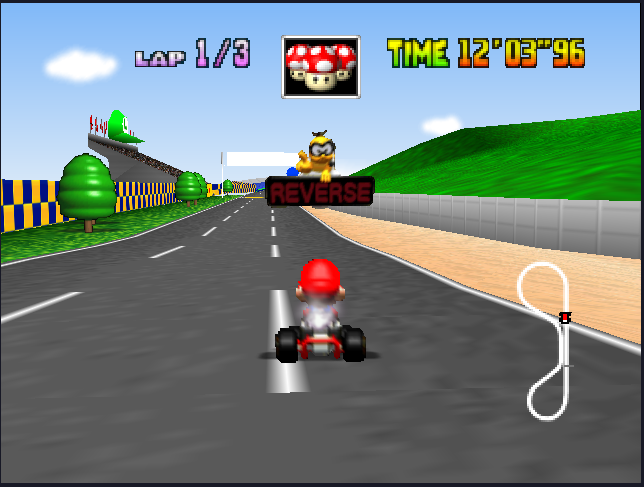
\includegraphics[width=0.8\linewidth]{images/demo.png}

   \caption{Example of run where agent spent most of time driving backwards}
   \label{fig:onecol}
\end{figure}

Therefore several changes have been made, mainly to the design of the state, action, and rewards, which have been described in this paper. However, they have yet to be tested and further changes and adjustments will be made. For example, more actions may be added or removed to improve performance, such as adding more defined left and right directions (eg. hard left and soft left) or removing the option to reverse and having the car auto-accelerate to simplify the problem. 

%%%%%%%%% REFERENCES
{\small
\bibliographystyle{ieee_fullname}
\bibliography{egbib}
}

\end{document}
